\chapter{Theoretical Background}
\label{cap-background}

As described in \textcite{fowler2018refactoring}, refactoring is a design improvement after writing a code. Refactoring opportunities may arise throughout the project's development regardless of how the project was designed, especially in systems developed by teams.

Refactoring seeks to remove code smells encountered in software development; when software becomes mature and evolves, two conflicts arise: i) the software needs to fulfill all requirements, and ii) The software's reusability. Implementing new functionality in software without refactoring is possible, but it will eventually take great effort \cite{Gamma2009}.

Refactoring can facilitate the implementation of new requirements, modularize overloaded classes, and find methods and unnecessary classes. Different types of refactoring exist, such as techniques or methods based on design patterns. \textcite{fowler2018refactoring} is one of the most known authors. He created a catalog separating the refactorings into seven (7) groups and making it available for consultation. Fowler's online catalog encompasses the refactorings described in his two books: Refactoring: Improving the Design of Existing Code \cite{fowler2018refactoring} and Refactoring: Ruby Edition \cite{fields2009refactoring}. 

Refactoring by designing pattern-based methods examines the source code for insertion points to apply patterns. This refactoring aims mainly at maintainability, readability, and reusability. Several authors propose their pattern-based refactoring methods, such as \textcite{cinneide2000automated}, \textcite{Gamma2009}, and \textcite{ouni2017more}.

This chapter has information about the research background. \Cref{sec-importance} discuss the importance of refactoring. \Cref{sec-methods} describes the application of refactoring. \Cref{sec-tools} exemplifies the refactoring methods and the explanations of its functionalities and tools. \Cref{sub-rmt} talks about the RMT functionality. \Cref{sub-architecture} describes the architecture of the tool. \Cref{subsub-internal} talks about the internal functionality of RMT. \Cref{sub-usage} shows how to use the tool. \Cref{subsub-limitation} discusses the limitations encountered using the tool. \Cref{sec-microservices} explain about microservices. \Cref{sec2-remarks} includes the final considerations.

\section{Importance of Software Refactoring}
\label{sec-importance}
\textcite{fowler2018refactoring} describes that the first step in refactoring is to create automated tests, such as unit tests. The tests help to avoid creating bugs by guaranteeing that the behavior does not change, as any code change could also change the code behavior. Humans may make mistakes and cause serious problems in production. In system production, maintainability is a significant factor that influences costs, and one of the proposed solutions to reduce it is to increase software quality. 

Refactoring can be applied to the development process to increase software quality, forcing the programmer to find bad smells (a characteristic of the code that indicates an issue) \cite{Wilking2007}. 
In the study of \textcite{szHoke2017empirical}, six systems were analyzed to verify the effectiveness of software refactoring aimed at maintainability. To obtain data before refactoring, \textcite{szHoke2017empirical} analyzed all systems using a code analyzer called the SourcerMeter tool based on the Columbus tool \cite{ferenc2002}. Refactorings were performed manually, and developers were informed of all the data and the list of problematic code fragments. 

In the study \textcite{szHoke2017empirical}, developers analyzed 2.5 million lines and performed 732 code revisions, of which 315 were refactorings and 1,273 refactoring operations. After finishing the analysis, \textcite{szHoke2017empirical} found that refactoring improved maintainability and that the tool improved 5 of the six systems tested. In conclusion, the study shows that refactoring improves maintainability, which helps to meet future software requirements.

\subsection{Methods to Apply refactoring}
\label{sub-methods}
As mentioned, we can apply refactoring techniques and methods based on design patterns. Refactoring by techniques is common and can be found in leading IDEs, such as Eclipse and IntelliJ, which provide automatic refactorings based on the model created by \textcite{fowler2018refactoring}. 

Several authors propose software refactoring methods applying patterns, each performed differently in refactorings using pattern-based design methods. Some of these authors are \textcite{liu2014automated}, \textcite{zafeiris2017automated}, \textcite{cinneide2000automated}, and \cite{ouni2017more}. 

These refactoring methods seek to find the point of insertion of the pattern in the source code. The technique searches for source code to find where to implement design patterns to improve code maintainability, readability, and reusability. 

Unlike technical refactoring, design pattern-based refactoring looks for parts of the code where a design pattern can be applied. Using a design pattern is very important because it makes the evolution of the software more natural and does not create problems when implementing new requirements. Several project patterns have different functionality, such as the factory method, proxy, observer, adapter, visitor, builder, and others \cite{Gamma2009}). 

As described in the mapping performed by \textcite{beluzzo2018abordagem}, several authors propose methods for refactorings based on design patterns. For example, in the Moore method and Minipatterns and Minitransformations, there is a tool for each implementation process. If the developer wants to refactor his source code, he has to run n tools, where n is the total number of methods.

The focus of refactoring by design patterns differs from refactoring by techniques. Refactoring by design patterns tries to find a way to make a system easy to "update." Software that is difficult to update can cost the company a lot in value and the need for new clients and competitiveness with other companies \cite{cinneide2000automated}.

The next section presents methods for detecting and applying design patterns described in the literature.

\subsection{Methods and Tools for Refactoring Based on Design Patterns}
\label{sec-tools}

As mentioned, \textcite{beluzzo2018abordagem} identified methods for detecting and involving design patterns as described in \Cref{tab-articles}.


\begin{tabframed}[!htbp]
\caption{Articles with design patterns methods}
\label{tab-articles}
\begin{tabularx}{\textwidth}{|e{}@{},{}@{}|p{3cm}|p{8cm}|c|c@{}|}
%% Cabeçalho da primeira página
\toprule%
\multicolumn{1}{|@{}c|}{\textbf{Key}}             &
\multicolumn{1}{c|}{\textbf{Author}}             &
\multicolumn{1}{c|}{\textbf{Title}}              &
\multicolumn{1}{c|}{\textbf{Year}}               &
\multicolumn{1}{c@{}|}{\textbf{Has Tool}}        \\
\midrule%
A1  & \citeauthor*{GAITANI201533}            & Automated refactoring to the Null Object design pattern                                                             & 2015 & Yes      \\
A2  & \citeauthor*{CHRISTOPOULOU20121201}    & Automated refactoring to the Strategy design pattern                                                                & 2012 & Yes      \\
A3  & \citeauthor*{zafeiris2017automated}           & Automated refactoring of super-class method invocations to the Template Method design pattern                       & 2017 & Yes      \\
A4  & \citeauthor*{CINNEIDE2015}             & A multi-objective refactoring approach to introduce design patterns and fix anti-patterns                           & 2015 & Yes      \\
A5  & \citeauthor*{cinneide2001automated}    & Automated application of design patterns: a refactoring approach                                                    & 2001 & Yes      \\
A6  & \citeauthor*{cinneide792644}           & A Methodology for the automated introduction of design patterns                                                     & 1999 & Yes      \\
A7  & \citeauthor*{mens972774}               & A declarative evolution framework for object-oriented design patterns                                               & 2001 & Yes      \\
A8  & \citeauthor*{sang1183003}              & An automated refactoring approach to design pattern-based program transformations in Java programs                  & 2002 & Yes      \\
A9  & \citeauthor*{Cinneide602499}           & Automated Software Evolution Towards Design Patterns                                                                & 2001 & Yes      \\
A10 & \citeauthor*{cinneide337612}           & Automated refactoring to introduce design patterns                                                                  & 2000 & Yes      \\
A11 & \citeauthor*{Liu2014}                  & Automated pattern-directed refactoring for complex conditional statements                                           & 2014 & No       \\
A12 & \citeauthor*{ram2004detecting}         & Detecting Intent Aspects from Code to Apply Design Patterns in Refactoring: An Approach Towards a Refactoring Tool  & 2004 & Yes      \\
A13 & \citeauthor*{hotta6178876}             & Identifying, tailoring and suggesting form template method refactoring Opportunities with program dependence graph. & 2012 & Yes      \\
A14 & \citeauthor*{rajesh1013988}            & JIAD: A tool to infer design patterns in refactoring                                                                & 2004 & Yes      \\
A15 & \citeauthor*{ouni2017more}             & MORE: A multi-objective refactoring recommendation approach to introducing design patterns and fixing code smells   & 2017 & Yes      \\
A16 & \citeauthor*{eden632834}               & Precise specification and automatic application of design patterns                                                  & 1997 & No       \\
A17 & \citeauthor*{kerievsky2005refactoring} & Refactoring to Patterns                                                                                             & 2008 & No       \\
A18 & \citeauthor*{kim7332467}               & Scripting parametric refactorings in java to retrofit design patterns                                               & 2015 & No       \\
A19 & \citeauthor*{kim2014scripting}         & Scripting Refactorings in Java to Introduce Design Patterns                                                         & 2014 & Yes      \\
A20 & \citeauthor*{juillerat4362900}         & Toward an implementation of the ”Form Template Method” Refactoring                                                  & 2007 & Yes      \\
A21 & \citeauthor*{ajouli6619484}            & Transformations between composite and visitor implementations in Java                                               & 2013 & Yes     \\
\bottomrule%
\end{tabularx}
\SourceOrNote{adapted from \textcite{beluzzo2018abordagem}}
\end{tabframed}
\FloatBarrier

Each article has methods to recognize design pattern insertions, but not every article has a tool to apply it, as described in \Cref{tab-articles}. \textcite{beluzzo2018abordagem} searched for the articles until 2018, when his work was published. A new search was conducted with the same search strings and libraries from 2019 to 2024; no new work was found.

Some steps should be taken to refactor the code and apply transformations, as refactoring is not a straightforward technique and may vary by who is using it. That is why the authors have taken different approaches to refactoring listed in \Cref{tab-refactoring}.

\begin{table}[!htbp]
\caption{Refactoring Types}%
\label{tab-refactoring}
\begin{tabularx}{\textwidth}{e{},{}@{}lX@{}}
\toprule%
\multicolumn{1}{@{}c}{\textbf{Keys}}  &
\multicolumn{1}{c@{}}{\textbf{Types}} \\
\midrule%
A15, A10, A9, A6, A5 & MiniTransformations                                        \\
A2, A11              & Conditional Expression Refactorings                        \\
A12, A14             & Intent Aspects Refactoring*                                \\
A18, A19             & Reflective Refactorings                                    \\
A4, A15, A21         & Composite to Visitor and Visitor to Composite Refactorings \\
A4, A7, A15          & Role based Refactorings                                    \\
\bottomrule%
\end{tabularx}
\SourceOrNote{adapted from \textcite{beluzzo2018abordagem}}
\end{table}
\FloatBarrier


A refactoring type is applied to the code for every work, as described in \Cref{tab-refactoring} and listed in \Cref{tab-refactoring}. Minitransformations are minitransformations that are simple modifications to the code. By grouping these transformations in the right way, a design pattern is created \cite{cinneide2001automated}.

Reflective refactoring is based on code reflections, a technique that allows the code to be changed on runtime. It is good to emphasize that there are no pre-refactoring implementations with reflections; they are a method to implement the refactorings \cite{beluzzo2018abordagem}. 

Role-based refactoring is defined by a group of roles corresponding to the pattern participants and applying those roles to the refactor, obtaining the design pattern \cite{mens972774}. 

Intent aspects are software susceptible to pattern refactoring, formed by a group of rules for each pattern\cite{ram2004detecting}. Composite to Visitor and Visitor to Composite focus only on the transition between each pattern \cite{beluzzo2018abordagem}. Finally, Conditional Expression Refactorings focus on the code's conditional expressions and conditional branches to refactor \cite{CHRISTOPOULOU20121201}.

As shown in \Cref{tab-articles}, most articles have tools developed to apply your specific method, working in an automatic or semi-automatic manner.

\begin{table}[!htbp]
\caption{Developed tools}%
\label{tab-tools}
\begin{tabularx}{\textwidth}{e{},{}@{}lX@{}}
\toprule%
\multicolumn{1}{@{}c}{\textbf{Keys}}  &
\multicolumn{1}{c@{}}{\textbf{Tools}} \\
\midrule%
A2, A3         & JDeodorant                   \\
A4             & MORE                         \\
A6, A7, A8, A9 & Prototype\textbf{*}          \\
A5, A10        & Design Pattern Tool          \\
A13            & Creios                       \\
A12, A15       & JIAD                         \\
A15            & MORE                         \\
A11, A19, A20  & Eclipse Plugin\textbf{*}     \\
A21            & JHotDraw                     \\
\bottomrule%
\end{tabularx}
\SourceOrNote{adapted from \textcite{beluzzo2018abordagem}}
\end{table}
\FloatBarrier

In \Cref{tab-tools}, the developed tools are listed by name; the row marked with an asterisk means that the tool is a prototype or an eclipse plugin; the other articles were created or updated of specific tools\cite{beluzzo2018abordagem}.

The tool creation is necessary because manual refactoring, the process some developers use, can introduce errors to the code and even change the system's functionality. This problem occurs because developers are not prepared to perform a refactoring \cite{ge2012reconciling}.

Manual refactoring requires reviewing the entire code and can take time. For this reason, tools facilitate the application of refactorings, which can identify bad smells or identify and refactor the source code, as created by \textcite{beluzzo2018abordagem}.

\textcite{beluzzo2018abordagem} performed a mapping to find refactoring techniques, and several tools have already been developed to perform refactorings. Such as Elbereth \cite{korman1998elbereth}, which automates some code extraction refactorings, encompassing method extraction (Extract Method), abstract superclasses, replacement of an existing class, and addition of a new subclass.

To improve the interaction with the user for the application of refactoring, \cite{murphy2008breaking} created a tool that is fast, resistant to errors, and pleasant to use. To make the tool enjoyable, they implemented markings in the code produced by rectangles, arrows, and coloring parts of the code. These three markings show the user cleanly where and what the problem is so that refactorings can be applied.
Some tools contain a graphical interface and iteration with the user, such as \textcite{rani2014detection}, where the intent is to detect bad smells. This tool was developed in C\# and finds terrible smells such as the long method, large class, lazy class, and comment lines. Discovering smells in code written in Java and .net. 

Many code refactoring tools are based on the catalog of refactorings created by \textcite{fowler2018refactoring}, as in the integrated development environment (IDE) (e.g., Eclipse, Netbeans, and IntelliJ). However, some authors utilize design pattern-based refactoring as in \cref{tab-tools}. Authors, such as \textcite{cinneide2000automated} and \textcite{CHRISTOPOULOU20121201} agree that automated refactoring reduces application time and can be more beneficial, as it allows less experienced developers to apply refactorings. They were making tools for this reason.

\textcite{murphy2008breaking}, together with eight software developers with different work experiences, used the GostFactor tool to assist in refactoring. They observed that this process decreased errors in the refactoring application by 23.3\%.

The RMT tool, as developed by \textcite{beluzzo2018abordagem}, facilitates the seamless integration of design pattern insertion and detection methods within a unified environment. This tool engages in an interactive process with the developer, providing foresight into the inherent changes after refactoring and concurrently evaluating the effectiveness of such refactoring in enhancing code quality. \textcite{sangeetha2019empirical} 's work, although it does not explain tool implementation, employs it for experimental verification and validation of the used techniques. The RMT is designed to support the implementation of any specified method \textcolor{red}{citar os métodos} \cite{beluzzo2018abordagem}.

\subsection{RMT}
\label{sub-rmt}

The RMT (Refactoring and Measurement Tool) was created to identify design pattern insertion points utilizing the methodologies implemented by \textcite{beluzzo2018abordagem}. \textcite{zafeiris2017automated} and \textcite{liu2014automated} are responsible for developing the implemented refactoring techniques. The developed approaches are, respectively, the refactoring of the Template Method pattern and the refactoring of the Strategy and Factory Method patterns. The \cref{fig-activity-rmt} illustrates the flow of the RMT tool without discriminating between implementations. The figure is divided into two distinct colors, each representing a unique request (thread) on hold by the client user and, consequently, by the intermediary service.

\begin{figure}[ht!]
\SetCaptionWidth{\textwidth}
\caption{Activity diagram for RMT}
\label{fig-activity-rmt}
\fontsize{3.8}{5}\selectfont
\includesvg[width =\textwidth]{Chapter-2/Figures/activity-rmt.svg}
\SourceOrNote{Own authorship (2024)}
\end{figure}
\FloatBarrier

The use activity diagram delineates the tool's functionality for the user. The client initiates the process by uploading the project and searching for potential candidates. Upon identification of any applicable methods, the corresponding metric is computed. Within the interface, the client can select a class for refactoring, if necessary, and subsequently execute the refactoring process. Without identified candidates, the process ends without proceeding to refactoring and metric computation.

\textcolor{red}{Pedro, aqui você arrumou o diagrama de caso de uso que a professor Simone Senger soliciou}.

In addition to applying the refactorings, the tool uses the CK metrics extractor \cite{ck}, which encompasses the metrics of the depth of the inheritance tree (PAH), the cyclomatic complexity (CC), and the size of the program in lines of code (TPLC). Upon selecting a project selected for refactoring, the metrics are applied to demonstrate the effects of refactoring on the user source code. The available external quality attributes are maintainability, reliability, and reusability.

\subsubsection{RMT Architecture}
\label{sub-architecture}

The architecture diagram in \cref{fig-architecture} starts with user iteration within the Client App, as it is isolated and runs independently since it is a Java desktop application; the communication can be only made with the Intermediary Service, which provides the communication between the user layer (Client) and the processing layer (Services). The Intermediary Service uses Hypertext Transfer Protocol (HTTP) requests to communicate to the subsequent Metrics and the Detection Service.

\textcite{beluzzo2018abordagem} model also proposes separating the services by region, which may offer better availability. This mitigation is accomplished by distributing services across multiple geographic regions (including distinct cities, states, and countries), thereby ensuring continuity of service and preventing total system failure in the event of a regional outage. The database is a global service that can be accessed from any region. \Cref{fig-architecture} represents the regional divisions of application services.

\begin{figure}[ht!]
\SetCaptionWidth{\textwidth}
\caption{RMT architecture diagram}
\label{fig-architecture}
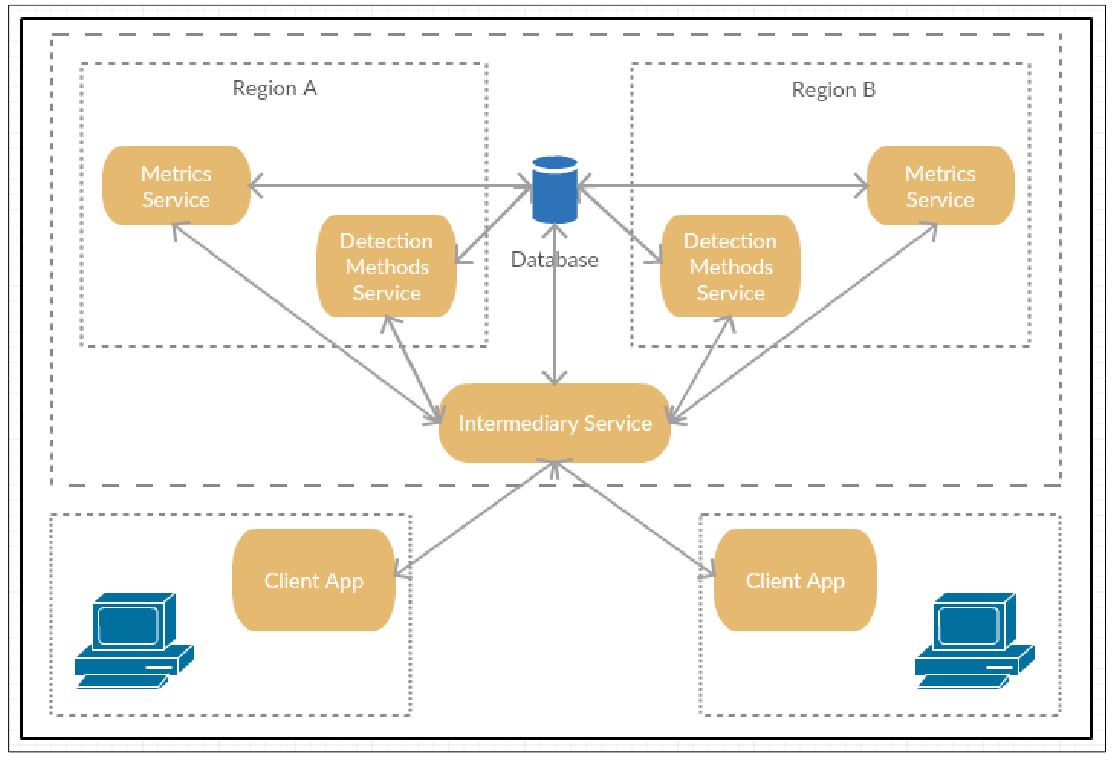
\includegraphics[width =\textwidth]{Chapter-2/Figures/schema.png}
\SourceOrNote{\textcite{beluzzo2018abordagem}}
\end{figure}
\FloatBarrier

\textcolor{red}{<<achei estranho o começo dessa frase>>} 

The intermediary service functions as a service registry, possessing detailed knowledge of every service across all regions and strategically selecting the optimal server for communication. At a high level, upon receiving a project from the user, the intermediary service engages with the detection service, which subsequently provides the refactoring candidates. Following this, the intermediary service requests the detection service to perform the refactoring on the identified candidates. Upon receiving the responses from the refactored candidates, the metrics service is invoked to compute the quality attributes. Ultimately, the intermediary service aggregates all pertinent information and formulates a response for the user.

\textcite{beluzzo2018abordagem} attempted to conceptualize an extensible tool, facilitating new implementations without experiencing substantial obstacles. However, he did not delineate a concrete process for extension.

\subsubsection{Internal structure}
\label{subsub-internal}

The architecture of a computational system is critical for its proper functionality; however, most intensive processing operations are executed within the services. An optimally designed service will operate efficiently with minimal memory and CPU resources, ensuring compatibility with small-scale computer instances. The methodology for selecting candidates for refactoring using RMT is illustrated in \Cref{fig-candidates}.

\begin{figure}[ht!]
\SetCaptionWidth{\textwidth}
\caption{Sequence Diagram to Find Refactoring Candidates}
\label{fig-candidates}
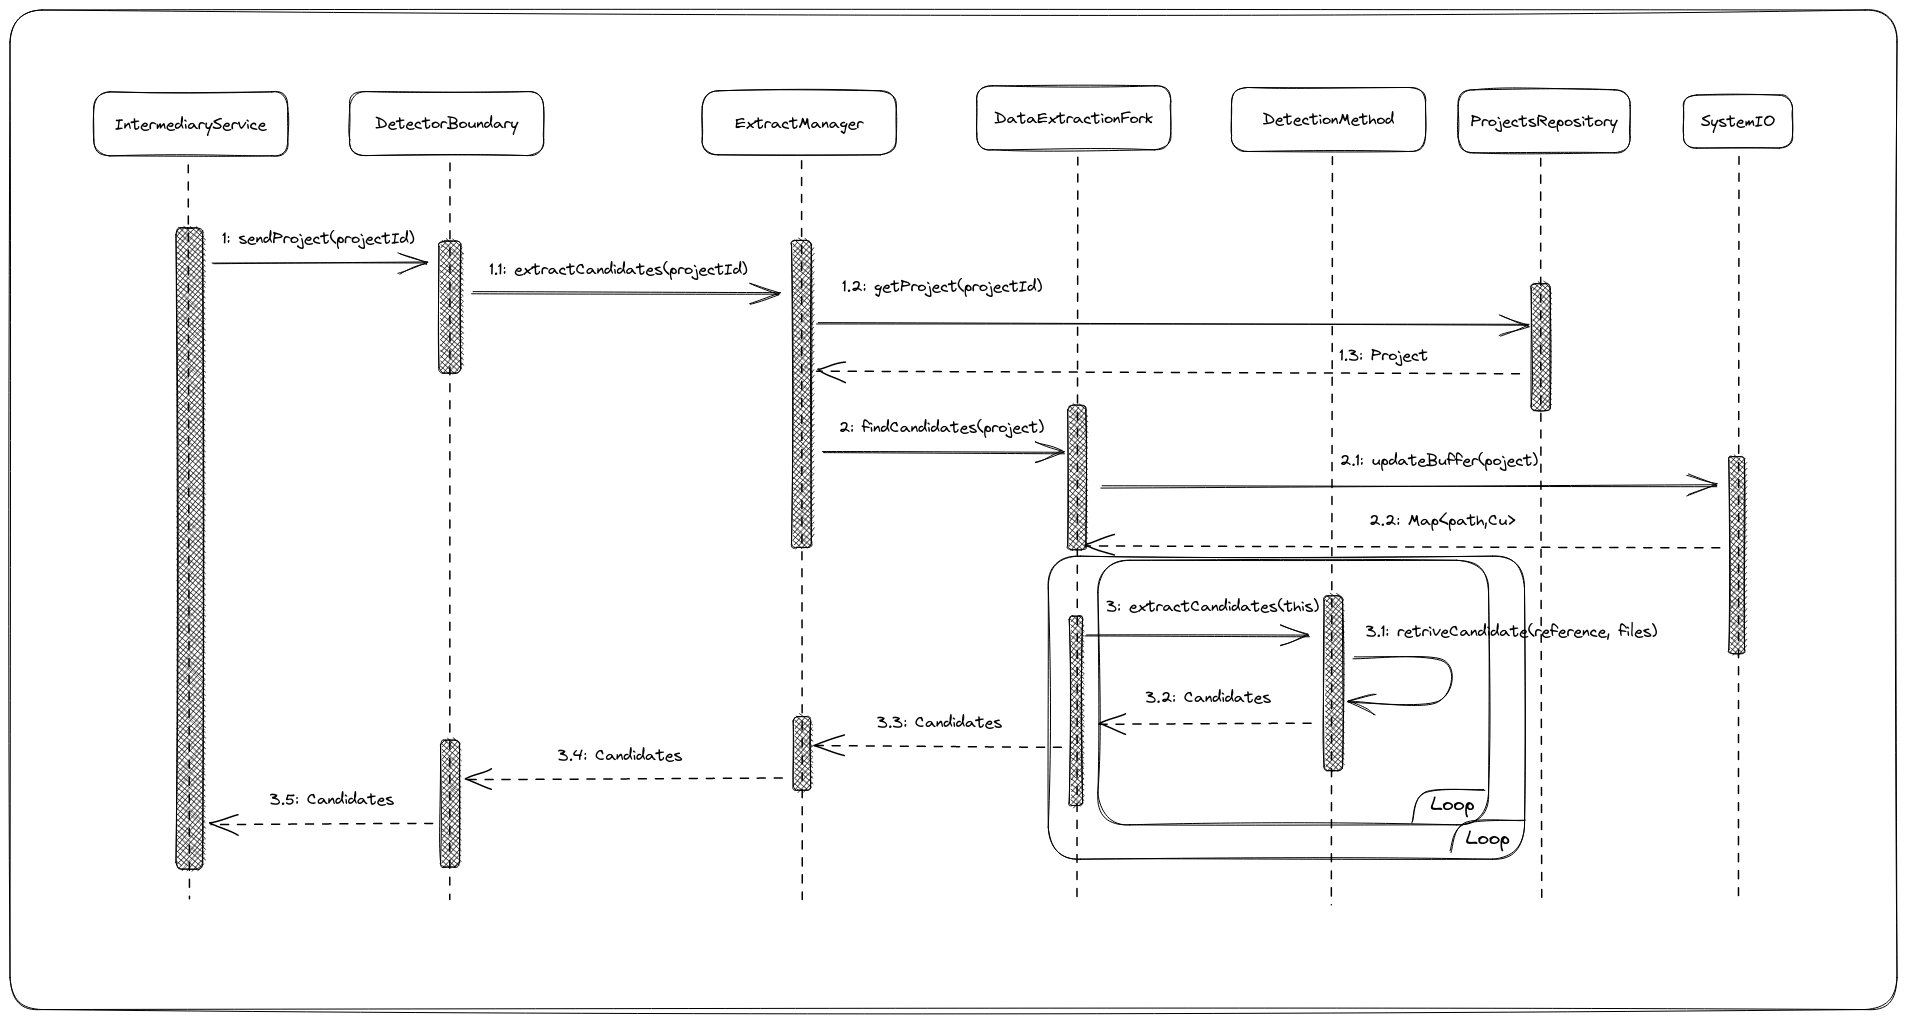
\includegraphics[width=160mm]{Chapter-2/Figures/candidates.png}
\SourceOrNote{Own authorship (2023)}
\end{figure}
\FloatBarrier

As described, the intermediary service communicates with the detection service after saving the project to the database and sends the project ID, as in Step 1.

The detection service receives an HTTP request on the \texttt{DetectionBoundary} class and, with the project ID, calls the \texttt{extractCandiates} method. The controller process occurs in Step 1.1.

The id is received by the \texttt{ExtractManager} class, which is the interface responsible for calling the \texttt{getProject} method to retrieve the project from the repository; the actions are represented by Step 1.2.

The \texttt{ProjectRepostiory} is an interface with database access that is used to retrieve project information along with the project zip file as \texttt{InputStream} in the \texttt{Project} entity, completing Step 1.3. Step 2 sends the retrieved project to the \texttt{DataExtractionFork}.

The \texttt{DataExtractionFork} has direct access to the system's input and output (io), saving the project and retrieving it immediately afterward. The project is saved as a zip file to be parsed as a \texttt{CompilationUnit} class (class representation of abstract syntax tree) and loaded into the memory to be sent to every implementation of the DetectionMethod as in Step 2.1.

The \texttt{DetectionMethod} is an interface that abstracts the functionality of a refactoring method. It receives an instance of the \texttt{DataExtactionFork} and iterates over every file to detect the possibility of designing the pattern insertion; the process results are returned to the intermediary service, finishing Steps 3.1 to 3.5.

If any candidate was detected, the intermediary service automatically calls the service of the detection to refactor those candidates as in \Cref{fig-refactoring}.

\begin{figure}[ht!]
\SetCaptionWidth{\textwidth}
\caption{Sequence Diagram for Refactoring Candidates}
\label{fig-refactoring}
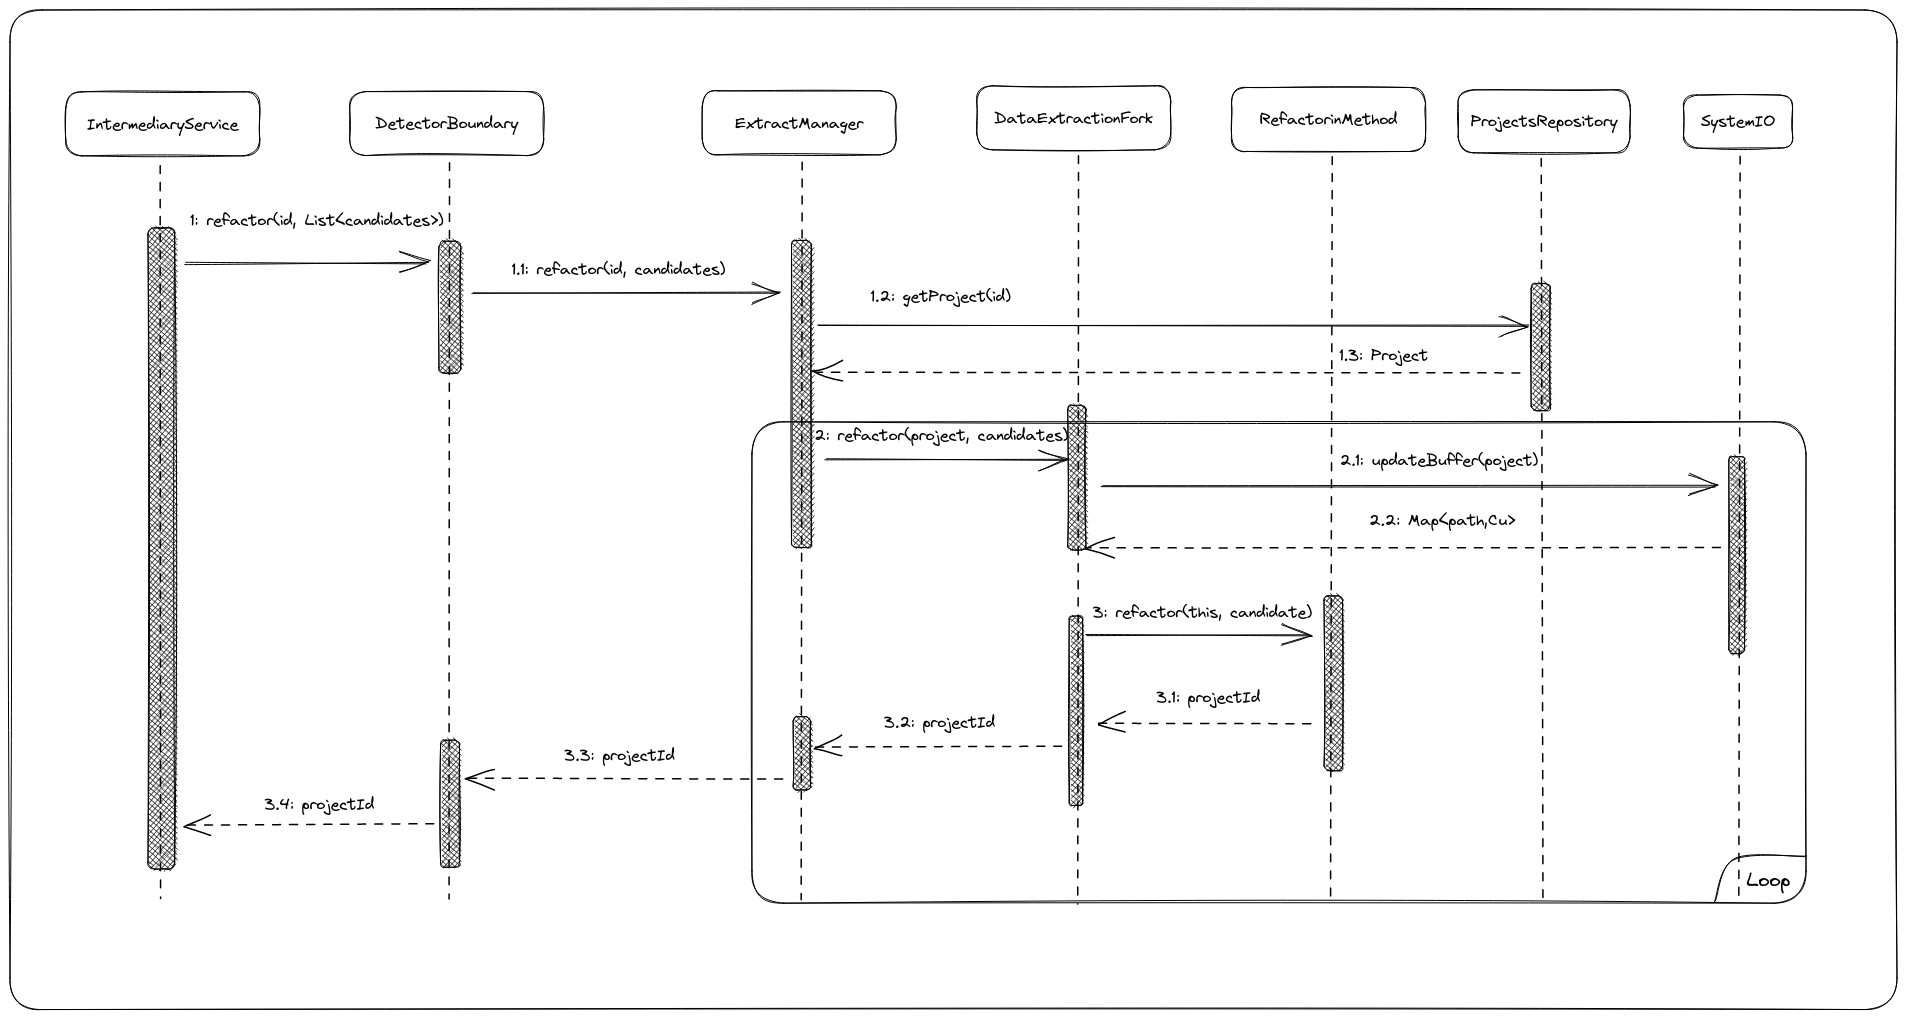
\includegraphics[width=160mm]{Chapter-2/Figures/refactoring.png}
\SourceOrNote{Own authorship (2023)}
\end{figure}
\FloatBarrier

\texttt{DetectionBoundry} class is the application controller, it recives the request to start the refactoring, within the request are the classes choose by the user to be refactored and the project ID, the information is send to the \texttt{ExtractManager} as Step 1.1.

The \texttt{ExtractManager} class has the same functionality as in \Cref{fig-candidates}, retrieving the project from the database by the \texttt{ProjectRepository} (Step 1.2); and then calling the \texttt{DataExtractionFork} class over a loop as Step 2.

 In Step 2.1, \texttt{DataExtractionFrok} has the same functionality as in \cref{fig-candidates}. However, every candidate in the project inflates the zip file and converts it to a \texttt{CompilationUnit} class to be refactored in Step 3. After refactoring has ended, the project ID is returned from 3.1 to 3.4.

\subsubsection{RMT Usage}
\label{sub-usage}

The main focus of explaining the usage of RMT is on the Client App, which is divided into three stages. The first step is to import the project, as shown in \Cref{fig-import}.

\begin{figure}[ht!]
\SetCaptionWidth{\textwidth}
\caption{Importing project on clientApp}
\label{fig-import}
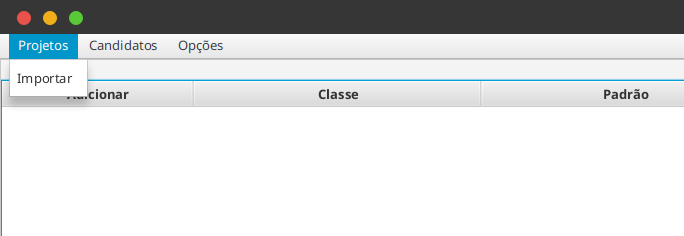
\includegraphics[width =100mm]{Chapter-2/Figures/import.png}
\SourceOrNote{Own authorship (2023)}
\end{figure}
\FloatBarrier

The second step is the project evaluation, giving feedback to the user, which can analyze additional information about the candidates for refactoring, such as class name, design pattern, and metrics, as shown in \Cref{fig-choose}.

\begin{figure}[ht!]
\SetCaptionWidth{\textwidth}
\caption{Selecting refactoring candidates}
\label{fig-choose}
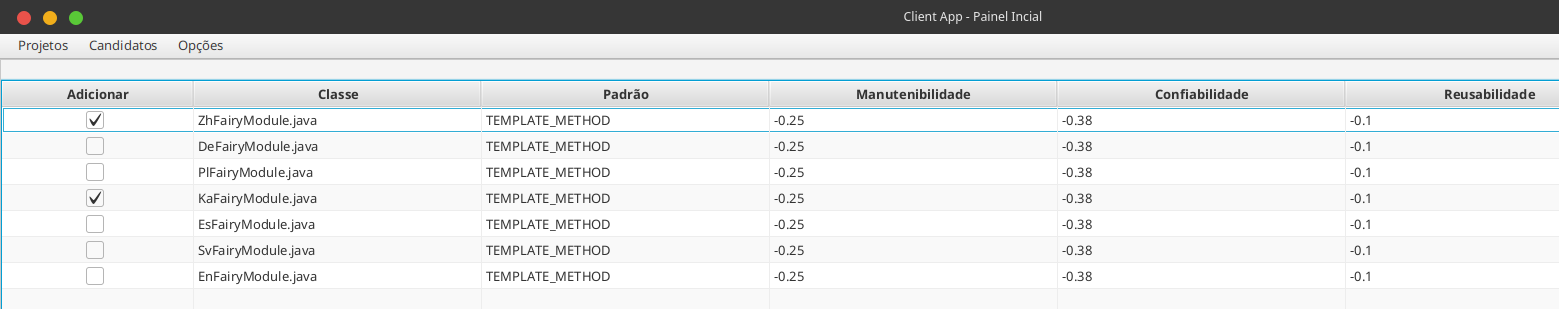
\includegraphics[width =\textwidth]{Chapter-2/Figures/choose.png}
\SourceOrNote{Own authorship (2023)}
\end{figure}
\FloatBarrier

In the third and last step, the user can choose the candidates to apply the refactoring after using it to a new project created and saved in a user-selected directory, as shown in \Cref{fig-refactor}.

\begin{figure}[ht!]
\SetCaptionWidth{\textwidth}
\caption{Applying refactoring to candidates}
\label{fig-refactor}
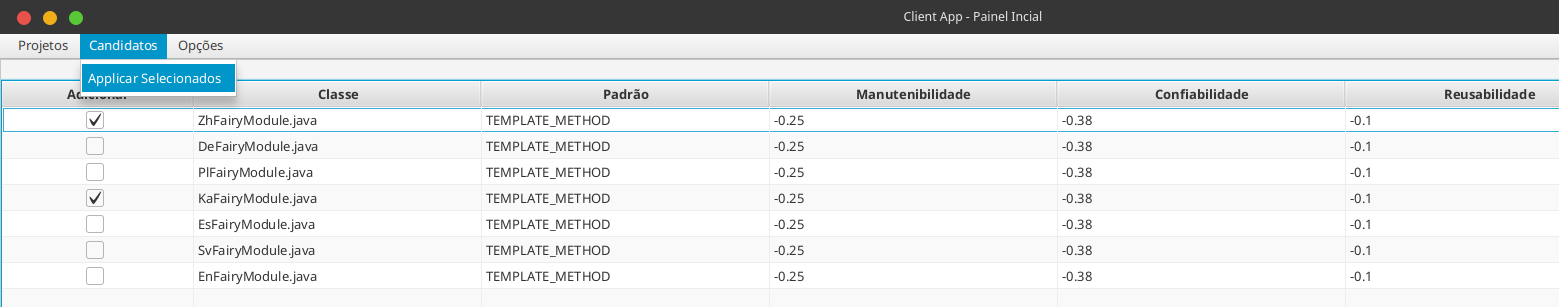
\includegraphics[width =\textwidth]{Chapter-2/Figures/refactor.png}
\SourceOrNote{Own authorship (2023)}
\end{figure}
\FloatBarrier

\subsubsection{RMT Limitations}
\label{subsub-limitation}
When testing the RMT, some limitations were noticed. The first limitation was the long time required to execute a project refactoring, which involved drilling down on the tool code to find the reason for the slowness. One section had strange behavior: starting a refactoring system, extracting a zip file, and parsing every file to memory to verify if it could be a refactoring candidate. The problem is that the parsing process is repeated for each file and is repeated even more when the candidate is refactored. Following the same idea, when the candidate is refactored, each refactoring step is saved on the filesystem, once again accessed, and parsed to retrieve the changes. The disk (filesystem) has expensive access and takes time; a better option is to handle all the access directly on the memory.

The blocking request issue manifests when many users concurrently access the tool, thereby saturating the available connections. Any new users will increase latency and may induce users to receive an error from the server as they have to wait until other processes are over to open space for a new connection. This problem mainly occurs because of the synchronous architecture on RMT based on an API manager (intermediary service) communicating with the other services via HTTP requests, holding the service thread until the call ends. This behavior could cause problems in other functionalities, such as the load balancer, service registry, and service discovery, which occurs because the service has no more threads to execute any code. It may crash or freeze. Since Java 8 is limited by the system threads, scaling vertically (upgrading the CPU) is the only way to support more clients. The downside of HTTP communication is that latency increases with the number of concurrent clients \cite{Cebeci2020DesignOA}. 

In the detection service, the Java Parser library \textcite{javaparser} is in versions that support only features up to Java 9 (the last release is Java 22). That was not a limitation when the tool was built but became a limitation as it ages. This limitation can be addressed by constantly updating the library.

Another limitation is related to the CK \textcite{ck} library used to calculate the metrics; the library code was copied to the tool code, making it difficult to update for new versions and take advantage of new metrics and features. 

The RMT shows two refactorings for the same design pattern and class. Therefore, the user has only the metrics to choose from, which will be applied; there are no other ways to explain the difference between the method to the user to make a better decision.

The tool currently lacks unit tests to ensure the logic implemented within the class is accurate. Such tests are instrumental in facilitating refactoring efforts, ensuring that while the code undergoes structural modifications, its intended functionality remains unchanged as long as the tests pass.

\section{Microservices Architecture}
\label{sec-microservices}
The microservices are used to create large and complex applications, as the model shown in \Cref{fig-architecture}, each application must be simple and independent. When services are connected and working together, they become a system. As discussed in \textcite{microservices-comuni}, the application is fault-tolerant and more controllable than a monolithic architecture.

There are many architectures, such as synchronous RMT and asynchronous ones. The synchronous services wait for the response before ending the process; they usually use a direct connection over Representational State Transfer (REST), Remote Procedure Call (RCP), etc. \cite{microservices-comuni}. To implement a retry on synchronous services, the caller service must handle the failure without terminating the connection.

Asynchronous services do not wait for a response; the communication is non-block, so the service does not wait for the answer to end the process; it can be achieved with queues as communication means. Some queue services are RabbitMQ, Apache Kafka, and Simple Service Queue (SQS), among others \cite{KARABEYAKSAKALLI2021111014}. Queue services have resilience-oriented characteristics, including the ability to persist unconsumed messages, thus ensuring that requests are not lost even if a service experiences downtime \cite{Cebeci2020DesignOA}.

\textcolor{red}{<<a frase seguinte eu não compreendi>>}

To continue improving system resilience, queue services incorporate mechanisms designed to facilitate message retry attempts. such as visibility timeout, which is the time that a message is only visible to one consumer. If the message is not processed by the end of the time, it becomes visible again, returns to the queue, and adds one to the retry count. The queue must be configured with a retry limit to avoid an infinite retry. A notable limitation is the potential for message duplication in scenarios involving operational failures \cite{ChenScalable}.

\textcolor{red}{<<achei que fatou comentar sobre trabalhos que usam esse tipo de arquiterua para criar suas ferramentas>> Pouco informação para a seção}

\section{Closing Remarks}
\label{sec2-remarks}
This chapter reported on the importance of refactoring, described the methods based on design patterns and refactoring tools, and explained some aspects of service architecture.

Refactoring is essential to keep the source code free from smells and to a quality standard. The main focus of refactoring is maintainability and reusability by maintaining the code as first designed and avoiding inserting new smells.

The importance of using a software refactoring tool was addressed to get the most out of refactoring without harming the work already done, highlighting that the RMT tool is the focus of this research.
The RMT tool integrates several methods for detecting and inserting design patterns in a single environment so that the application developer can apply them to their source code without using several refactoring tools.

There are many types of software architecture, but we discuss the abilities of the async and sync applications, bringing both upsides and downsides. This work used snowballing to ensure that no other tool, such as RMT, was used, and the results are presented in the next chapter.